\documentclass[a4paper, 12pt]{article}

\usepackage[T2A]{fontenc}
\usepackage[utf8]{inputenc}
\usepackage[english,russian]{babel}
\usepackage[left=15mm, top=19mm, right=15mm, bottom=20mm, nohead, nofoot]{geometry}


\usepackage{hyperref}
\usepackage{graphicx}
\graphicspath{{pictures/}}
\DeclareGraphicsExtensions{.pdf,.png,.jpg}
\usepackage{wrapfig}
\usepackage{afterpage}
\usepackage{fancyhdr}
\usepackage{longtable}
\pagestyle{fancy}
\usepackage{amsmath, amsfonts, amssymb, amsthm, mathtools}

\usepackage{graphicx, wrapfig, subcaption, setspace, booktabs}
\usepackage[protrusion=true, expansion=true]{microtype}
\usepackage[english]{babel}
\usepackage{sectsty}
\usepackage{url, lipsum}
\setcounter{tocdepth}{5}
\setcounter{secnumdepth}{5}



\title{Московский Физико-Технический Институт}
\author{Кафедра общей физики \\ Вопрос по выбору \\ Термодинамика}
\begin{document}
	\maketitle
\thispagestyle{empty}
	\begin{center}
		\rule{\linewidth}{0.5mm} \\[0.4cm]
	{ \Huge\bfseries Сопло Лаваля \\ [0.4cm] }
		\rule{\linewidth}{0.5mm} \\[0.4cm]
	\end{center}	
\begin{minipage}{0.6\textwidth}
	\begin{flushleft} \large
		\emph{Автор:}\\
		Маллаев Руслан\\
		Группа: Б02-005
	\end{flushleft}
\end{minipage}
\begin{center}
\end{center}

\maketitle
\thispagestyle{empty}
\newpage
\fancyhead[L] {Сопло Лаваля}

\mbox

\section*{Содержание:}
\begin{enumerate}
	\item Что такое сопло Лаваля?
	\item История появления сопла Лаваля;
	\item Уравнение неразрывности потока;
	\item Уравнение Бернулли;
	\item Устройство сопла Лаваля;
	\item Рассчет параметров для истечения по соплу Лаваля;
	\item Функционирование в среде;
	\item Применение сопла Лаваля;
	\item Вывод;
	\item Литература;
\end{enumerate}

\newpage
\mbox 

\section*{Что такое сопло Лаваля?}
\textbf{Сопло Лаваля} — газовый канал особого профиля, разгоняющий проходящий по нему газовый поток до сверхзвуковых скоростей. Сопло представляет собой канал, сужающийся в середине. В простейшем случае такое сопло может состоять из пары усечённых конусов, сопряжённых узкими концами (Рис.1).
\begin{figure}[h!]
    \begin{center}
    \includegraphics[width=0.6\textwidth]{pictur/ris1.png}
    \end{center}
    \caption{Сопло Лаваля}
    \end{figure}
\section*{История появления сопла Лаваля.}
Сопло Лаваля было предложено шведским изобретателем Густафом де Лавалем в 1890 году. Оно состоит из пары усеченных конусов сопряженных узкими  горловинами.  Такую конфигурацию, необычную для того времени, Лаваль получил методом проб и ошибок. Когда он направил струю пара из расширяющегося конуса на колесо турбины, то число оборотов её вала резко возросло. Турбиностроение перешло на новый технический уровень. Идея сопла Лаваля была востребована временем, поэтому она нашла сразу применение. Спустя некоторое время эту идею стали применять в ракетостроении, первым, кто это сделал, стал Р.Х.Годдард.\\

Рассмотрим уравнение неразрывности потока и уравнение Бернулли для дальнейшего изучения сопла Лаваля.
\section*{Уравнение неразрывности потока.}
\subsection*{Основные понятия:}
\begin{enumerate}
	\item \textbf{Площадью живого сечения потока} называют площадь сечения потока, приведенную нормально к направлению линии тока, т.е. перпендикулярно движению струйки жидкости. Живое сечение может быть ограничено твердыми стенками полностью или частично.
	\item \textbf{Расходом потока} называется количество жидкости, протекающей через поперечное сечение в единицу времени. Если рассматривать поток жидкости, представляющий собой

\newpage
\mbox
\\

совокупность большого числа элементарных струек, то очевидно, общий расход жидкости для всего потока в целом представляет собой сумму расходов всех отдельных струек.
\end{enumerate}
Данное уравнение основывается на законе постоянства массы, т.е.
\[
m=const.
\]
Количество (масса) газа, проходящего в единицу времени через поперечное сечение трубы (расход газа) равно $Q=\rho\upsilon{S}$, где $S$-площадь сечения, $\rho$-плотность вещества, $\upsilon$-характерная скорость вещества. Эта величина должна оставаться постоянной вдоль всей трубы:
\[
Q=\rho\upsilon{S}=const.
\eqno(1)
\]

\begin{figure}[h!]
    \begin{center}
    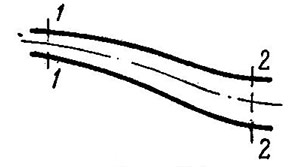
\includegraphics[width=0.6\textwidth]{pictur/2.jpg}
    \end{center}
    \caption{Сопло Лаваля}
\end{figure}
Обратимся к рисунку 2. Отделим сечениями 1-1 и 2-2 некоторый отрезок элементарной струйки. Расход газа, проходящего через сечение 1-1 $Q_1=\rho\upsilon_{1}S_1$, расход газа, проходящего через сечение 2-2 $Q_2=\rho\upsilon_{2}S_2$. Так как $Q=const$, то $Q_1=Q_2$ $\Rightarrow$ $\upsilon_1S_1=\upsilon_2S_2$ $\Rightarrow$
\[
\frac{\upsilon_1}{\upsilon_2}=\frac{S_2}{S_1}
\eqno(2)
\]
Из соотношения $(2)$ видим, что максимальные скорости достигаются при минимальных сечениях.\\
\section*{Уравнение Бернулли.}

\textbf{Стационарное (установившееся) течение жидкости} - это течение, при котором в каждой точке пространства, занятого жидкостью, скорость течения остается постоянной по времени. \textbf{Линия тока} - линии, касательные к которым указывают на направление вектора скорости в точке касания в данный момент времени. При стационарном движении жидкости они остаются неизменными и совпадают с траекториями частиц жидкости.\\

Уравнение Бернулли гласит, что вдоль линии тока в поле силы тяжести остается постоянно:
\[
\frac{\upsilon^2}{2}+i+gz=const,
\eqno(3)
\]
где $i=\frac{P}{\rho}+u=c_{p}T$ - тепловая функция (удельная энтальпия), $u$ - внутренняя энергия единицы массы газа.

\newpage
\mbox

\section*{Устройство сопла Лаваля}
Обратимся к рисунку 1. Сопло Лаваля представляется собой трубу, которая имеет вид песочных часов. Оно служит для ускорения газового потока проходящего через него до скоростей выше скорости звука. \\

При анализе течения газа в сопле Лаваля принимаются следующие упрощающие допущения:
\begin{enumerate}
	\item Газ считается идеальным;
	\item Газовый поток является изоэнтропным (то есть имеет постоянную энтропию, силы трения и диссипативные потери не учитываются) и адиабатическим (то есть теплота не подводится и не отводится);
	\item Газовое течение является стационарным и одномерным, то есть в любой фиксированной точке сопла все параметры потока постоянны во времени и меняются только вдоль оси сопла, причём во всех точках выбранного поперечного сечения параметры потока одинаковы, а вектор скорости газа всюду параллелен оси симметрии сопла;
	\item Массовый расход газа одинаков во всех поперечных сечениях потока;
	\item Влияние всех внешних сил и полей (в том числе гравитационного) пренебрежимо мало;
	\item Ось симметрии сопла совпадает с пространственной координатой $x$.\\
\end{enumerate}	

Введем понятие числа Маха: $M=\dfrac{\upsilon}{\upsilon_{\text{зв}}}$, где $\upsilon$ - локальная скорость, $\upsilon_{\text{зв}}$ - локальная скорость звука. 

Прологарифмируем выражение $(1)$, а затем его продифференцируем:
\[
ln(\rho)+ln(\upsilon)+ln(S)=ln(const)
\]
\[
\frac{d\rho}{\rho}+\frac{d\upsilon}{\upsilon}+\frac{dS}{S}=0.
\eqno(4)
\]

Из уравнения Бернулли для стационарного потока (с пренебрежением послем силы тяжести) получим:
\[
\frac{\upsilon^2}{2}+\frac{P}{\rho}+u=const;
\]
\[
u=c_{v}T;
\]
По определению показатель адиабаты $\gamma=\dfrac{c_{p}}{c_{v}}$. Соотношение Майера $c_{p}-c_{v}=\dfrac{R}{\mu}$ $\Rightarrow$ $c_{v}=\dfrac{R}{\mu(\gamma -1)}$. Из уравнения состояния $P=\dfrac{\rho}{\mu}RT$ $\Rightarrow$
\[
i=\frac{\gamma}{\gamma -1}\frac{P}{\rho}
\eqno(5)
\]
Принимая во внимание уравнение $(5)$, получим:

\newpage
\mbox

\[
\frac{\upsilon^2}{2}+\frac{\gamma}{\gamma -1}\frac{P}{\rho}=const
\eqno(6)
\]
Продифференцируем уравнение $(6)$:
\[
\upsilon{d\upsilon}+\frac{\gamma}{\gamma -1}\frac{\rho{dP}-Pd\rho}{\rho^2}=0
\eqno(7)
\]
Так как $\upsilon_{\text{зв}}^2=\dfrac{dP}{d\rho}$ $\Rightarrow$ $dP=\upsilon_{\text{зв}}^2d\rho$. Учтем так же, что $\upsilon_{\text{зв}}^2=\gamma\dfrac{P}{\rho}$, то $P=\dfrac{\rho\upsilon_{\text{зв}}^2}{\gamma}$. Подставим получившиеся соотношения в $(7)$ и получим:
\[
\frac{d\rho}{\rho}=-\frac{\upsilon{d\upsilon}}{\upsilon_{\text{зв}}^2}.
\eqno(8)
\]
Подставим выражение $(8)$ в выражение $(4)$:
\[
\frac{dS}{S}+\frac{d\upsilon}{\upsilon}\left(1-\frac{\upsilon^2}{\upsilon_{\text{зв}}^2}\right)=0
\]
Окончательный вид:
\[
\frac{d\upsilon}{\upsilon}\left(1-M^2\right)=-\frac{dS}{S}
\eqno(9)
\]
Из выражения $(9)$ можно сделать вывод о том, что если $M<1$, то знак $d\upsilon$ противоположен знаку $dS$, если $M>1$, то знак $d\upsilon$ совпадает со знаком $dS$.\\

Это означает, что скорость дозвукового потока при сужении сопла растет и уменьшается в случае его расширения. В сверхзвуковом потоке, наоборот, при расширении сопла скорость увеличивается, поток ускоряется. Максимальная скорость в самой узкой части сопла не превышает скорости звука в заданном месте. Именно на этом принципе и основывается сопло Лаваля. Таким образом в сопле есть скорость дозвукового потока и сверхзвукового потока.

\section*{Рассчет параметров для истечения по соплу Лаваля}
Обратимся к уравнению Бернулли $(3)$. Предположим, что на одной линии тока есть точка, в которой скорость газа равна нулю. Тогда уравнение Бернулли можно записать в виде:
\[
i+\frac{\upsilon^2}{2}=i_0,
\eqno(10)
\]
где $i_0$ - энтальпия в точке $\upsilon=0$.\\

Из уравнения $(10)$ видно, что скорость $\upsilon$ больше в тех местах, где тепловая функция $i$ меньше. Энтальпия - термодинамическая функция $\Rightarrow$ $di=Tds+vdP$. Процесс истечения считаем изоэнтропическим $\Rightarrow$ $di=vdP=dP/\rho$. Так как $\rho>0$, то $di$ и $dP$ имеют одинаковые знаки и потому изменение $i$ и $p$ направлено всегда в одну сторону. Следовательно, можно сказать, что вдоль линии тока скорость всегда падает с увеличением давления, и наоборот.

Выясним характер изменения плотности потока жидкости $j=\rho\upsilon$. Уравнение Эйлера для одномерного случая:
\[
\upsilon\frac{d\upsilon}{dx}=-\frac{1}{\rho}\frac{dP}{dx}
\eqno(11)
\]

\newpage
\mbox

\[
\upsilon{d\upsilon}+\frac{dP}{\rho}=0
\]
Снова учтем, что $dP=\upsilon_{\text{зв}}^2d\rho$, и получим:
\[
\frac{d\rho}{d\upsilon}=-\frac{\rho\upsilon}{\upsilon_{\text{зв}}};
\]
\[
\frac{dj}{d\upsilon}=\rho\left(1-\frac{\upsilon^2}{\upsilon_{\text{зв}}^2}\right)
\eqno(12)
\]
Из уравнения $(12)$ видно, что по мере возрастания скорости вдоль линии тока плотность потока возрастает до тех пор, пока скорость остается дозвуковой. В области же сверхзвукового движения плотность потока падает с увеличением скорости и обращается в нуль при $\upsilon=\upsilon_{max}$. Это существенное различие между до- и сверхзвуковыми стационарными потоками можно объяснить следующим образом. В дозвуковом потоке линии тока сближвются друг с другом в направлении увеличения скорости. При сверхзвуковом же движении линии тока расходятся по мере увеличения скорости. Поток $j$ имеет максимальное значение $j_{*}$ в точке, в которой скорость газа равна местному значению скорости звука $j_{*}=\rho_{*}\upsilon_{\text{зв}*}$. Скорость $\upsilon_{*}=\upsilon_{\text{зв}*}$ называют критичекой скоростью.\\

Мы рассматриваем термодинамический идеальный газ. У такого газа теплоемкость является постоянной величиной, поэтому такой газ частно называют политропным. Для него применимо уравнение состояний:
\[
PV=\frac{P}{\rho}=\frac{RT}{\mu};
\]
Внутрення энергия политропного газа:
\[
u=c_{v}T=\frac{PV}{\gamma -1}=\frac{\upsilon_{\text{зв}}^2}{\gamma(\gamma -1)};
\]
Тепловая функция (энтальпия):
\[
i=c_{p}T=\frac{\gamma{PV}}{\gamma -1}=\frac{\upsilon_{\text{зв}}^2}{\gamma -1};
\eqno(13)
\]
Тогда энтропия газа:
\[
s=c_{v}ln\left(\frac{P}{\rho^{\gamma}}\right)=c_{p}ln\left(\frac{P^{\frac{1}{\gamma}}}{\rho}\right);
\]
Из общего курса физики мы знаем, что максимальная скорость истечения газа достигается при истечении в вакуум и определяется по формуле:
\[
\upsilon_{max}=\upsilon_{\text{зв0}}\sqrt{\frac{2}{\gamma -1}}
\]
Уравнение Бернулли для критической скорости можно записать в виде:
\[
\frac{\upsilon_{*}^2}{\gamma(\gamma -1)}+\frac{\upsilon_{*}^2}{2}=\frac{\upsilon_{\text{зв}0}^2}{\gamma -1};
\]
Получим связь между скоростью звука в критической точке и скорость звука в сопле при входе:
\[
\upsilon_{*}=\upsilon_{\text{зв}0}\sqrt{\frac{2}{\gamma +1}};
\eqno(14)
\]

\newpage
\mbox
\\

Процесс адиабатический $\Rightarrow$ по адиабате Пуассона 
\[
\rho=\rho_{0}\left(\frac{T}{T_{0}}\right)^{\frac{1}{\gamma-1}}, P=P_{0}\left(\frac{\rho}{\rho_{0}}\right)^{\gamma};
\eqno(15)
\]
Подставив в уравнение Бернулли выражения $(13)$, получим
\[
T=T_{0}\left(1-\frac{\gamma -1}{\gamma +1}\frac{\upsilon^2}{\upsilon_{*}^2}\right);
\eqno(16)
\]
Аналогично применяя $(15)$ получим:
\[
\rho=\rho_{0}\left(1-\frac{\gamma -1}{\gamma +1}\frac{\upsilon^2}{\upsilon_{*}^2}\right)^{\frac{1}{\gamma -1}};
\eqno(17)
\]
\[
P=P_{0}\left(1-\frac{\gamma -1}{\gamma +1}\frac{\upsilon^2}{\upsilon_{*}^2}\right)^{\frac{\gamma}{\gamma -1}};
\eqno(18)
\]
Тогда выражения для критической точки:
\[
T_{*}=\frac{2T_{0}}{\gamma +1}, P_{*}=P_{0}\left(\frac{2}{\gamma +1}\right)^{\frac{\gamma}{\gamma -1}}, \rho_{*}=\rho_{0}\left(\frac{2}{\gamma +1}\right)^{\frac{1}{\gamma -1}}
\]
Определим теперь скорость истечения газа из сопла Лаваля:
\[
\upsilon=\upsilon_{\text{зв}0}\sqrt{\frac{2}{\gamma -1}\left(1-\left(\frac{P}{P_{0}}\right)^{\frac{\gamma -1}{\gamma}}\right)};
\]
\[
\upsilon_{\text{зв}0}^2=\gamma\frac{P_{0}}{\rho_0};
\]
\[
\upsilon=\sqrt{\frac{2\gamma}{\gamma -1}\frac{P_0}{\rho_0}\left[1-\left(\frac{P}{P_{0}}\right)^{\frac{\gamma -1}{\gamma}}\right]}=\sqrt{\frac{2\gamma}{\gamma -1}\frac{RT_0}{\mu}\left[1-\left(\frac{P}{P_{0}}\right)^{\frac{\gamma -1}{\gamma}}\right]};
\eqno(19)
\]
где $P_0$-давление на входе в сопло, $P$-давление газа на выходе из сопла, $T_0$-температура на входе в сопло.

\section*{Функционирование в среде.}
При работе сопла Лаваля в непустой среде (чаще всего речь идет об атмосфере) сверхзвуковое течение может возникнуть только при достаточно большом избыточном давлении газа на входе в сопло по сравнению с давлением окружающей среды. При $P_0$(давление на входе сопло)=$P^{0}$(атмосферное давление) движения газа нет. 

При достаточно высоком значении $P_0$ давления хватает ровно настолько, чтобы к выходу из сопла давление плавно выровнялось с атмосферным. Вместе с непрерывным падением давления непрерывно растет скорость. Режим при котором в сверхзвуковом сопле происходит непрерывное уменьшение давления от $P_0$ до $P^{0}$ называется расчетным. Для конкретного сопла существует единственное значение , при котором оно работает в расчетном режиме и $P$(давление на выходе сопла)=$P^{0}$.

Режимы, при которых относительное давление слишком велико, чтобы обеспечить сверхзвуковую скорость именно на срезе сопла называют нерасчетными, а сопла, работающие в этих режимах – перерасширенными.

\newpage
\mbox

\begin{figure}[h!]
	\center{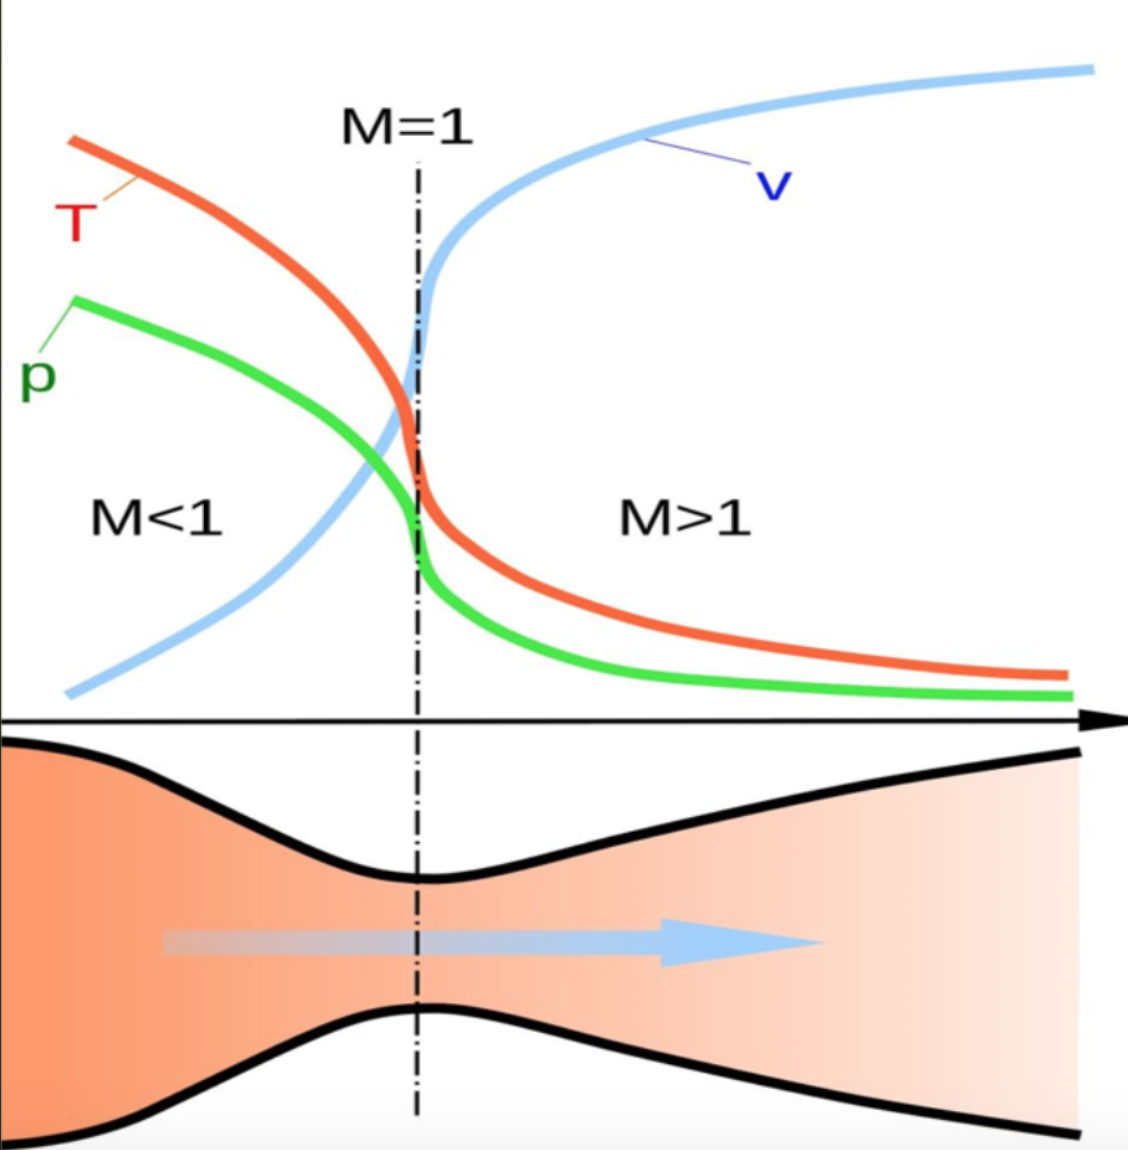
\includegraphics[width = 0.45 \linewidth]{pictur/Screenshot 2021-06-01 at 08.31.53.png}}
	\caption{Графики зависимостей величин от числа Маха.}
\end{figure}

\section*{Применение сопла Лаваля.}
По причине высокой эффективности ускорения газового потока, нашли практическое применение сопла Лаваля. В ракетном двигателе сопло Лаваля впервые было использовано генералом М. М. Поморцевым в 1915 году. В ноябре 1915 года в Аэродинамический институт обратился генерал М. М. Поморцев с проектом боевой пневматической ракеты.

\begin{figure}[h!]
	\center{\includegraphics[width = 0.45 \linewidth]{pictur/ф.png}}
	\caption{Ракета Поморцева.}
\end{figure}

Пневматическая ракета генерала Поморцева состоит из стальной трубы, один конец которой (B) закрыт, а друтой (а) имеет сопло. Отверстие (a) закрыто пробкой, которая при помощи остроумного приспособления может быть открыта в любой момент. Воздух в ракете сжимался до 100-125 атмосфер, и в нее вводили бензин или эфир, чтобы образовать взрывчатую смесь, или помещали в нее порох. 


\section*{Вывод.}
Мы исследовали сложное устройство сопло Лаваля, получили значения критических параметров и скорость выходящего газа, а также узнали об его применении.

\newpage
\mbox

\section*{Литература.}
\begin{enumerate}
	\item Ландау Л. Д., Лифшиц Е. М. Глава X. Одномерное движение сжимаемого газа.  \S 97. Истечение газа через сопло // Теоретическая физика. — Т. 6. Гидродинамика.$[1]$
	\item Ландау Л. Д., Лифшиц Е. М. Глава lX. Ударные волны. \S 83. Стационарный поток сжимаемого газа // Теоретическая физика. — Т. 6. Гидродинамика.$[2]$
\end{enumerate}
\end{document}